%This work is licensed under the Creative Commons License Attribution 4.0 International (CC-BY 4.0)
%https://creativecommons.org/licenses/by/4.0/legalcode
\documentclass[rgb]{standalone}
\usepackage{tkz-euclide}
\definecolor{myorange}{hsb}{0.0833, 1, 0.8}
\definecolor{mygreen}{hsb}{0.3333, 1, 0.8}
\definecolor{myblue}{hsb}{0.5833, 1, 0.8}
\definecolor{mymagenta}{hsb}{0.8333, 1, 0.8}
\begin{document}
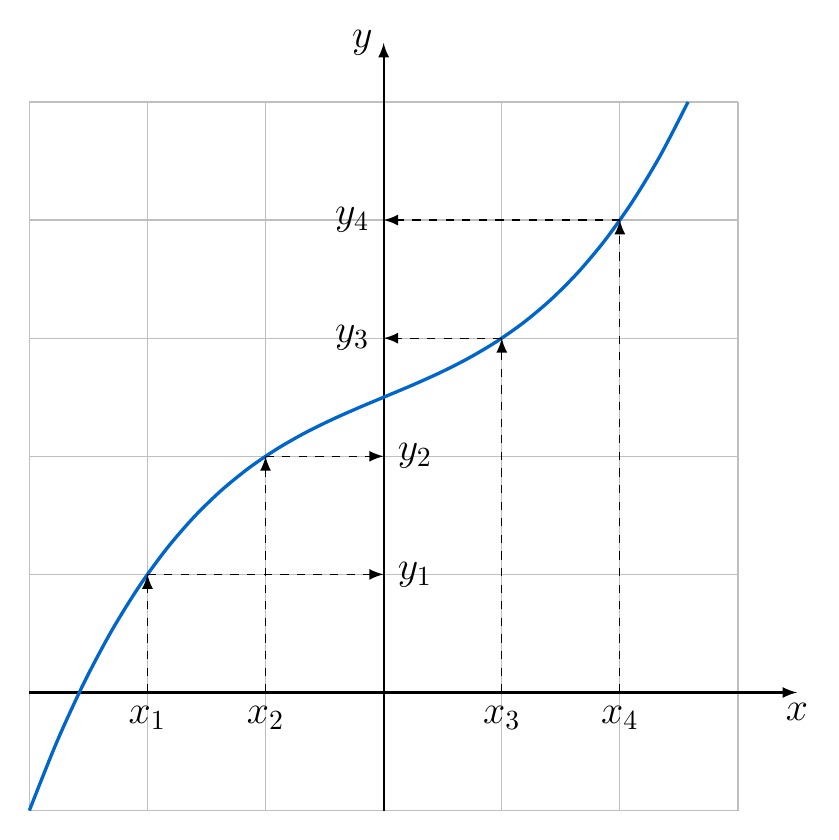
\begin{tikzpicture}[scale=1.5, font=\Large]
	% Coordinate system
	\tkzInit[xmin=-3,xmax=3,ymin=-1,ymax=5]
	\tkzGrid[color=lightgray]
	\tkzDrawX[thick,label=$x$]
	\tkzDrawY[thick,label=$y$]
	% Graph
	\draw[very thick,domain={-3}:{2.5771}, smooth, variable=\x, myblue] plot ({\x}, {2.5+1/12*\x*\x*\x+5/12*\x});
	\draw[dashed, -latex] (-2,0) -- (-2,1);
	\draw[dashed, -latex] (-1,0) -- (-1,2);
	\draw[dashed, -latex] (1,0) -- (1,3);
	\draw[dashed, -latex] (2,0) -- (2,4);
	\draw[dashed, -latex] (-2,1) -- (0,1);
	\draw[dashed, -latex] (-1,2) -- (0,2);
	\draw[dashed, -latex] (1,3) -- (0,3);
	\draw[dashed, -latex] (2,4) -- (0,4);
	% Labels
	\node[below=0.5mm] at (-2,0){$x_1$};
	\node[below=0.5mm] at (-1,0){$x_2$};
	\node[below=0.5mm] at (1,0){$x_3$};
	\node[below=0.5mm] at (2,0){$x_4$};
	\node[right=0.5mm] at (0,1){$y_1$};
	\node[right=0.5mm] at (0,2){$y_2$};
	\node[left=0.5mm] at (0,3){$y_3$};
	\node[left=0.5mm] at (0,4){$y_4$};
\end{tikzpicture}	
\end{document}